\documentclass[conference]{IEEEtran}

\usepackage{cite}
\usepackage{graphicx}
\usepackage{booktabs}
\usepackage{multirow}
\usepackage{array}
\usepackage{url}
\usepackage[hidelinks]{hyperref}

\title{RTDL: A Python-Hosted Ray-Tracing DSL with Bounded Reproduction of the RayJoin Workload Family}

\author{\IEEEauthorblockN{Anonymous Submission}}

\begin{document}
\maketitle

\begin{abstract}
RTDL (Ray-Tracing Domain Language) is a Python-hosted domain-specific language and compiler/runtime stack for
non-graphical ray-tracing workloads. This paper presents the current RTDL
solution through the RayJoin workload family as a bounded, externally checked,
multi-backend vertical slice. The system combines a Python authoring surface, a
backend-independent compiled-kernel representation, a native C/C++ oracle, and
controlled execution backends for Intel Embree and NVIDIA OptiX, with Vulkan
retained as a provisional backend. We evaluate RTDL against the workload and
artifact structure of the RayJoin paper using accepted bounded packages on a
Linux host and an external PostGIS reference. The resulting package closes the
tractable RayJoin experiment surface under an explicit bounded/analogue rule: available
families are validated across PostGIS, the native oracle, Embree, and OptiX;
synthetic scalability figures are reproduced as bounded analogues; and dataset
families with unstable or unavailable public acquisition paths are deferred
explicitly rather than overclaimed. The paper reports the RTDL design, the
evaluation methodology, the resulting correctness and performance evidence, and
the precise boundaries that separate bounded closure from paper-identical
reproduction.
\end{abstract}

\begin{IEEEkeywords}
domain-specific language, ray tracing, spatial joins, Embree, OptiX, PostGIS,
RayJoin, reproducibility
\end{IEEEkeywords}

\section{Introduction}

Ray-tracing hardware and software stacks are increasingly useful outside
graphics, but programming them directly still imposes a heavy systems burden on
application authors. Spatial join workloads are a clear example: the algorithmic
idea may be natural, yet the actual implementation often requires direct
management of acceleration structures, ray payloads, launch parameters, runtime
plumbing, and numerical boundary behavior. RTDL addresses that problem by
raising the programming surface to a compact kernel language while preserving a
backend path capable of executing RayJoin-style workloads across CPU and GPU
targets.

The current RTDL project is broader than a single application, but RayJoin is
its first serious target because the workload family is large enough to stress
the language/runtime boundary and structured enough to admit rigorous external
checks. This paper therefore does not present RTDL as a finished general system.
Instead, it presents a bounded, trustworthy vertical slice: a Python-hosted
language, a compiler/runtime pipeline, and a multi-backend evaluation package
that mirrors the RayJoin paper structure as far as current stable data and
infrastructure allow.

The main contribution of this paper is not a claim of paper-identical
reproduction. Rather, the contribution is a bounded reproduction package with
explicit fidelity labels and external correctness checks. RTDL now supports
accepted bounded closure for representative RayJoin-style workloads across a
native C/C++ oracle, Embree, OptiX, and PostGIS on selected real-data packages.
It also supports bounded analogues of the RayJoin scalability and overlay
surfaces. Dataset families whose public acquisition paths are unstable or
unavailable are deferred explicitly.

In summary, this paper makes four contributions:
\begin{enumerate}
\item It describes RTDL as a Python-hosted language and compiler/runtime system
for non-graphical ray-tracing applications, using RayJoin as the current
validation slice.
\item It documents a trusted execution stack consisting of a native semantic
oracle, controlled Embree and OptiX runtimes, and a PostGIS external checker.
\item It presents a bounded RayJoin experiment package covering LSI, PIP, and
overlay-seed analogue workloads across accepted available families.
\item It states precisely what has been reproduced, what is only an analogue,
and what remains deferred because of unavailable public data.
\end{enumerate}

\section{Background and Problem Setting}

RayJoin demonstrates that ray-tracing techniques can accelerate spatial joins,
but it also exposes the implementation burden of direct backend programming.
RTDL is motivated by the same application class while aiming to decouple kernel
semantics from backend-specific realization. In the current repo, the whole
project vision includes multiple backend families, but the validated slice is
intentionally narrower: RayJoin-style workloads executed through a native
oracle, Embree, and OptiX, with Vulkan retained only as a provisional path.

The evaluation surface mirrored from RayJoin includes three workload families
that matter directly for the current paper:
\begin{itemize}
\item \textbf{LSI}: line-segment intersection style joins,
\item \textbf{PIP}: point-in-polygon style joins,
\item \textbf{Overlay}: currently represented in RTDL as an
\textit{overlay-seed analogue}, not full polygon overlay materialization.
\end{itemize}

For this work, RayJoin Figure~13 and Figure~14 are represented as bounded
synthetic analogues, while RayJoin Table~3, Table~4, and Figure~15 are
represented through accepted bounded packages on stable and available dataset
families.

\section{Related Work}

\subsection{Spatial Join Systems}

RayJoin is the closest direct comparison point for this paper because RTDL is
explicitly evaluated against its workload family, artifact structure, and
reporting surfaces~\cite{rayjoin}. PostGIS remains the most important external
reference in the current RTDL evaluation because it provides a widely used
industrial spatial database with indexed spatial predicates and well-understood
geometry semantics~\cite{postgis}. GeoSpark SQL represents a different design
point: it exposes SQL-level spatial operations on top of a distributed
Spark/Hive execution substrate rather than a backend-portable kernel
language~\cite{geosparksql}. Other widely used distributed spatial systems, such
as SpatialHadoop and Apache Sedona, occupy the same broad system class even
though they expose different storage and execution tradeoffs~\cite{spatialhadoop,sedona}.
RTDL differs from all of these classes of systems. It is
not a database, and it is not a paper-specific one-off implementation. Instead,
it aims to express non-graphical ray-tracing workloads through a constrained
kernel language and then lower them into multiple execution backends while
keeping explicit correctness contracts.

\subsection{Compiler and DSL Context}

RTDL also relates to compiler-backed domain-specific systems such as
Halide~\cite{halide} and TVM~\cite{tvm}. Those systems separate high-level
computation intent from lower-level schedule or backend realization and are
therefore important precedents for RTDL's own authored-kernel to backend-plan
split. The difference is domain focus. Halide and TVM center image-processing
and tensor-operator pipelines, whereas RTDL centers geometric candidate
generation, refine predicates, and emitted join rows. The relevant design
pressure is therefore not only optimization, but exact spatial semantics across
heterogeneous backends.

\subsection{Ray-Tracing Runtime Context}

At the runtime layer, RTDL builds on ray-tracing infrastructure rather than
reimplementing traversal from scratch. Embree provides the validated CPU
ray-tracing kernel framework~\cite{embree}, while OptiX provides the accepted
GPU execution path in this paper~\cite{optix}. RTDL's contribution is not a new
traversal engine. The contribution is the language/runtime boundary, the native
oracle, and the bounded multi-system evidence package built on top of these
runtimes.

\section{RTDL Design}

\subsection{Language Surface}

RTDL is authored from Python through a constrained kernel DSL. A user writes a
kernel by declaring typed inputs, traversal intent, refine predicates, and
output fields. The intent is that authors specify workload meaning rather than
backend launch details. The same language surface currently supports six
implemented workloads in the repository, but the RayJoin-facing slice of this
paper focuses on LSI, PIP, and overlay.

\subsection{Compiled Representation and Lowering}

RTDL lowers authored kernels into a compiled-kernel representation that
separates language semantics from backend realization. The lowering path remains
RayJoin-oriented in the current codebase: it maps geometry roles, candidate
generation, refine predicates, and emitted rows into backend-specific execution
plans. This allows the same kernel to execute against a semantic oracle, a CPU
Embree runtime, and a GPU OptiX runtime.

\subsection{Execution Backends}

The accepted backends for this paper are:
\begin{itemize}
\item \textbf{Native C/C++ oracle}: the current semantic ground truth for
accepted results.
\item \textbf{Embree}: the strongest validated CPU backend in the repo.
\item \textbf{OptiX}: the bounded, controlled GPU backend validated on the
Linux workstation in Table~\ref{tab:environment}.
\end{itemize}

The Vulkan backend remains in the repository but is explicitly excluded from the
accepted paper package because it is still provisional.

\section{Methodology}

\subsection{Correctness Method}

The correctness story is intentionally layered. The native C/C++ oracle is the
internal ground truth. Embree and OptiX are checked against that oracle. For
accepted bounded real-data packages, PostGIS provides an external industrial
reference. PostGIS queries are executed with indexed GiST-assisted plans rather
than brute-force SQL. For PIP, PostGIS positive-hit queries are expanded into
the same full-matrix RTDL truth semantics before parity comparison.

The accepted PIP parity path is also more specific than a generic manual
point-in-polygon implementation. After the Goal~50 external comparison exposed
remaining boundary/topology mismatches, the accepted RTDL refine path adopted
GEOS-backed prepared-polygon \texttt{covers(point)} semantics for the native
oracle and Embree, and the accepted OptiX overlay result was observed on a
GEOS-enabled build on the validated Linux host~\cite{geos}. This detail matters
because the paper claims exact bounded parity with PostGIS on the accepted
packages, not merely approximate geometric agreement.

Parity is checked at the emitted-row level. In the accepted underlying
artifacts, each system produces a canonical row order, and the final row stream
is hashed with SHA-256. This paper therefore includes only cases whose final
accepted artifacts already established exact hash-level agreement across the
compared systems.

\subsection{Evidence Policy}

This paper uses only accepted artifacts from the repository's audited goal
history. A case is counted here only if it is already accepted and honestly
scoped. The paper therefore distinguishes:
\begin{itemize}
\item \textbf{done-bounded}: accepted bounded analogue or bounded package,
\item \textbf{deferred-unavailable}: excluded because the public acquisition
path is unstable or unavailable,
\item \textbf{not claimed}: paper-identical or nationwide statements that the
current repo does not justify.
\end{itemize}

All reported timings and parity statements in this paper come from the accepted,
final unified artifacts in the repository's audited goal history. Earlier
provisional or superseded measurements are intentionally excluded here.

\subsection{Experimental Environment}

Table~\ref{tab:environment} summarizes the host environment for the accepted
bounded package. All accepted four-system runs in this paper were executed on
the same Linux validation workstation.

\begin{table}[t]
\caption{Execution environment for the accepted bounded four-system package.}
\label{tab:environment}
\centering
\begin{tabular}{p{0.25\columnwidth}p{0.61\columnwidth}}
\toprule
Item & Value \\
\midrule
Host class & Linux validation workstation \\
OS & Ubuntu 24.04.4 LTS \\
CPU & Intel Core i7-7700HQ \\
Memory & about 15\,GiB \\
GPU & NVIDIA GeForce GTX 1070 \\
Driver & 580.126.09 \\
CPU RT backend & Embree 4.3.0 \\
GPU RT backend & OptiX 9.0.0 \\
External checker & local PostgreSQL/PostGIS on the same host \\
GEOS role & exact prepared-polygon \texttt{covers(point)} path for accepted PIP parity \\
\bottomrule
\end{tabular}
\end{table}

\subsection{Packages Used In This Paper}

The strongest accepted bounded package in the current repo consists of:
\begin{itemize}
\item County $\bowtie$ Zipcode on \texttt{top4\_tx\_ca\_ny\_pa},
\item BlockGroup $\bowtie$ WaterBodies on \texttt{county2300\_s10},
\item bounded LKAU $\bowtie$ PKAU on \texttt{sunshine\_tiny},
\item bounded LKAU $\bowtie$ PKAU overlay-seed analogue.
\end{itemize}

These packages were validated on the same Linux validation workstation.
The bounded LKAU $\bowtie$ PKAU package was staged from live OSM Overpass way
geometry and then frozen as the accepted bounded Australia slice~\cite{overpass}.

\subsection{Overlay-Seed Contract}

RTDL's current overlay result is not a materialized polygon geometry. The
accepted overlay row schema is instead an \emph{overlay-seed analogue} with
four columns:
\texttt{left\_polygon\_id},
\texttt{right\_polygon\_id},
\texttt{requires\_lsi}, and
\texttt{requires\_pip}.
This schema records whether a polygon pair requires line-segment intersection
refine, point-in-polygon refine, or both, and it is the exact surface compared
against PostGIS in the accepted bounded overlay package.

\section{Results}

\subsection{External Four-System Closure on Accepted Real-Data Packages}

Table~\ref{tab:four-system-main} summarizes the strongest accepted real-data
packages across PostGIS, the native oracle, Embree, and OptiX.

\begin{table*}[t]
\caption{Accepted bounded four-system results on the main real-data packages. Reported times are the accepted artifact timings carried forward from the final audited package reports; they are not averages across a new paper-only rerun. The Hits column is applicable only to PIP rows.}
\label{tab:four-system-main}
\centering
\small
\setlength{\tabcolsep}{4pt}
\begin{tabular}{p{0.29\textwidth}lrrr rrr}
\toprule
Package & Workload & Rows & Hits & PostGIS (s) & Native Oracle (s) & Embree (s) & OptiX (s) \\
\midrule
County $\bowtie$ Zipcode \texttt{top4\_tx\_ca\_ny\_pa} & LSI & 107513 & --- & 34.0323 & 89.3365 & 80.2707 & 53.2900 \\
County $\bowtie$ Zipcode \texttt{top4\_tx\_ca\_ny\_pa} & PIP & 16352128 & 7817 & 0.4300 & 24.4170 & 16.8128 & 19.2551 \\
BlockGroup $\bowtie$ WaterBodies \texttt{county2300\_s10} & LSI & 216 & --- & 0.2320 & 0.2286 & 0.2228 & 0.8933 \\
BlockGroup $\bowtie$ WaterBodies \texttt{county2300\_s10} & PIP & 71176 & 197 & 0.0084 & 0.1496 & 0.1172 & 0.6477 \\
\bottomrule
\end{tabular}
\end{table*}

For all four rows in Table~\ref{tab:four-system-main}, the correctness relation
is:
\begin{quote}
PostGIS $=$ native C oracle $=$ Embree $=$ OptiX
\end{quote}

This is the strongest accepted evidence in the current repo because it combines
external database truth with internal multi-backend agreement.

\subsection{Bounded Lakes/Parks Closure}

RTDL also closes a bounded lakes/parks analogue on Australia:

\begin{table}[t]
\caption{Accepted bounded LKAU $\bowtie$ PKAU package on \texttt{sunshine\_tiny}.}
\label{tab:lkau}
\centering
\small
\setlength{\tabcolsep}{4pt}
\begin{tabular}{p{0.34\columnwidth}rrrr}
\toprule
Workload & Rows & PostGIS (s) & Embree (s) & OptiX (s) \\
\midrule
LSI & 15 & 0.0623 & 2.1286 & 0.5072 \\
PIP & 73920 (22 hits) & 0.0041 & 0.0571 & 0.3844 \\
Overlay-seed analogue & 73920 & 0.2285 & 0.0850 & 0.5674 \\
\bottomrule
\end{tabular}
\end{table}

The LKAU package is explicitly bounded and derived from live OSM way geometry.
It is not continent-scale Australia-family closure. However, it is sufficient to
close the first accepted four-system overlay-seed analogue row in the project.
The corresponding native-oracle times are 1.9138\,s for LSI, 0.0915\,s for
PIP, and 5.1447\,s for the overlay-seed analogue.

\subsection{Scalability Analogues}

The RayJoin Section~5.6 style scalability surfaces are closed as bounded
analogues:
\begin{itemize}
\item RayJoin Figure~13: LSI query time and throughput under synthetic scaling,
\item RayJoin Figure~14: PIP query time and throughput under synthetic scaling.
\end{itemize}

These are accepted as \emph{done-bounded}, not paper-scale reproductions. They
remain valuable because they preserve experiment structure while staying within
the project's repeatable bounded execution budget.

In the accepted repo package, these analogues are driven by deterministic
synthetic scaling generators rather than the original full RayJoin data volume.
They preserve the same experiment shape---query time and throughput under
controlled scale-up---while remaining within the validated bounded execution
budget of the current project.

\begin{figure*}[t]
\centering
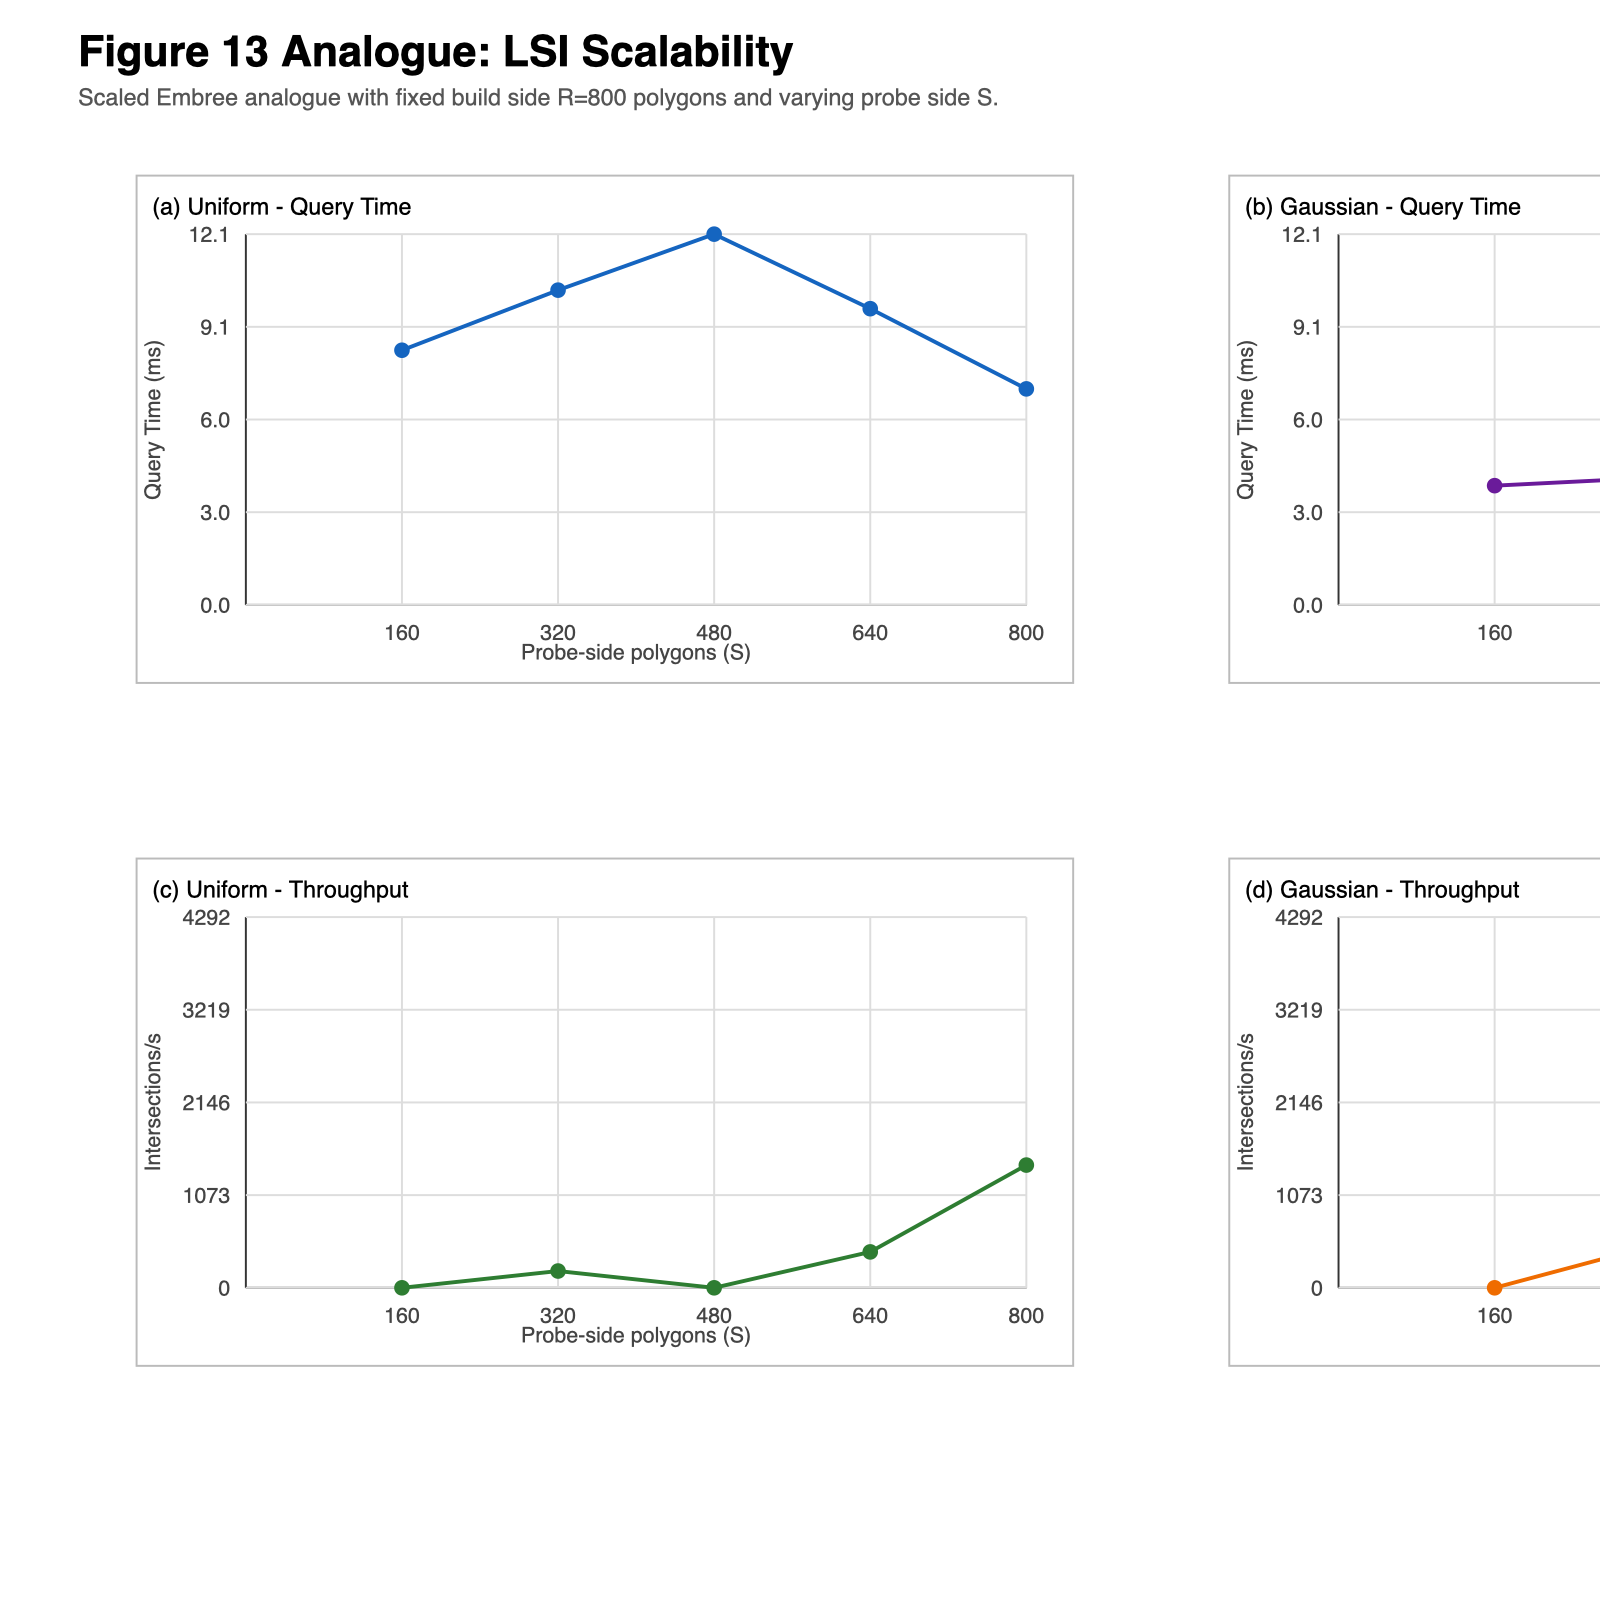
\includegraphics[width=0.48\textwidth]{figures/figure13_lsi_scalability.png}
\hfill
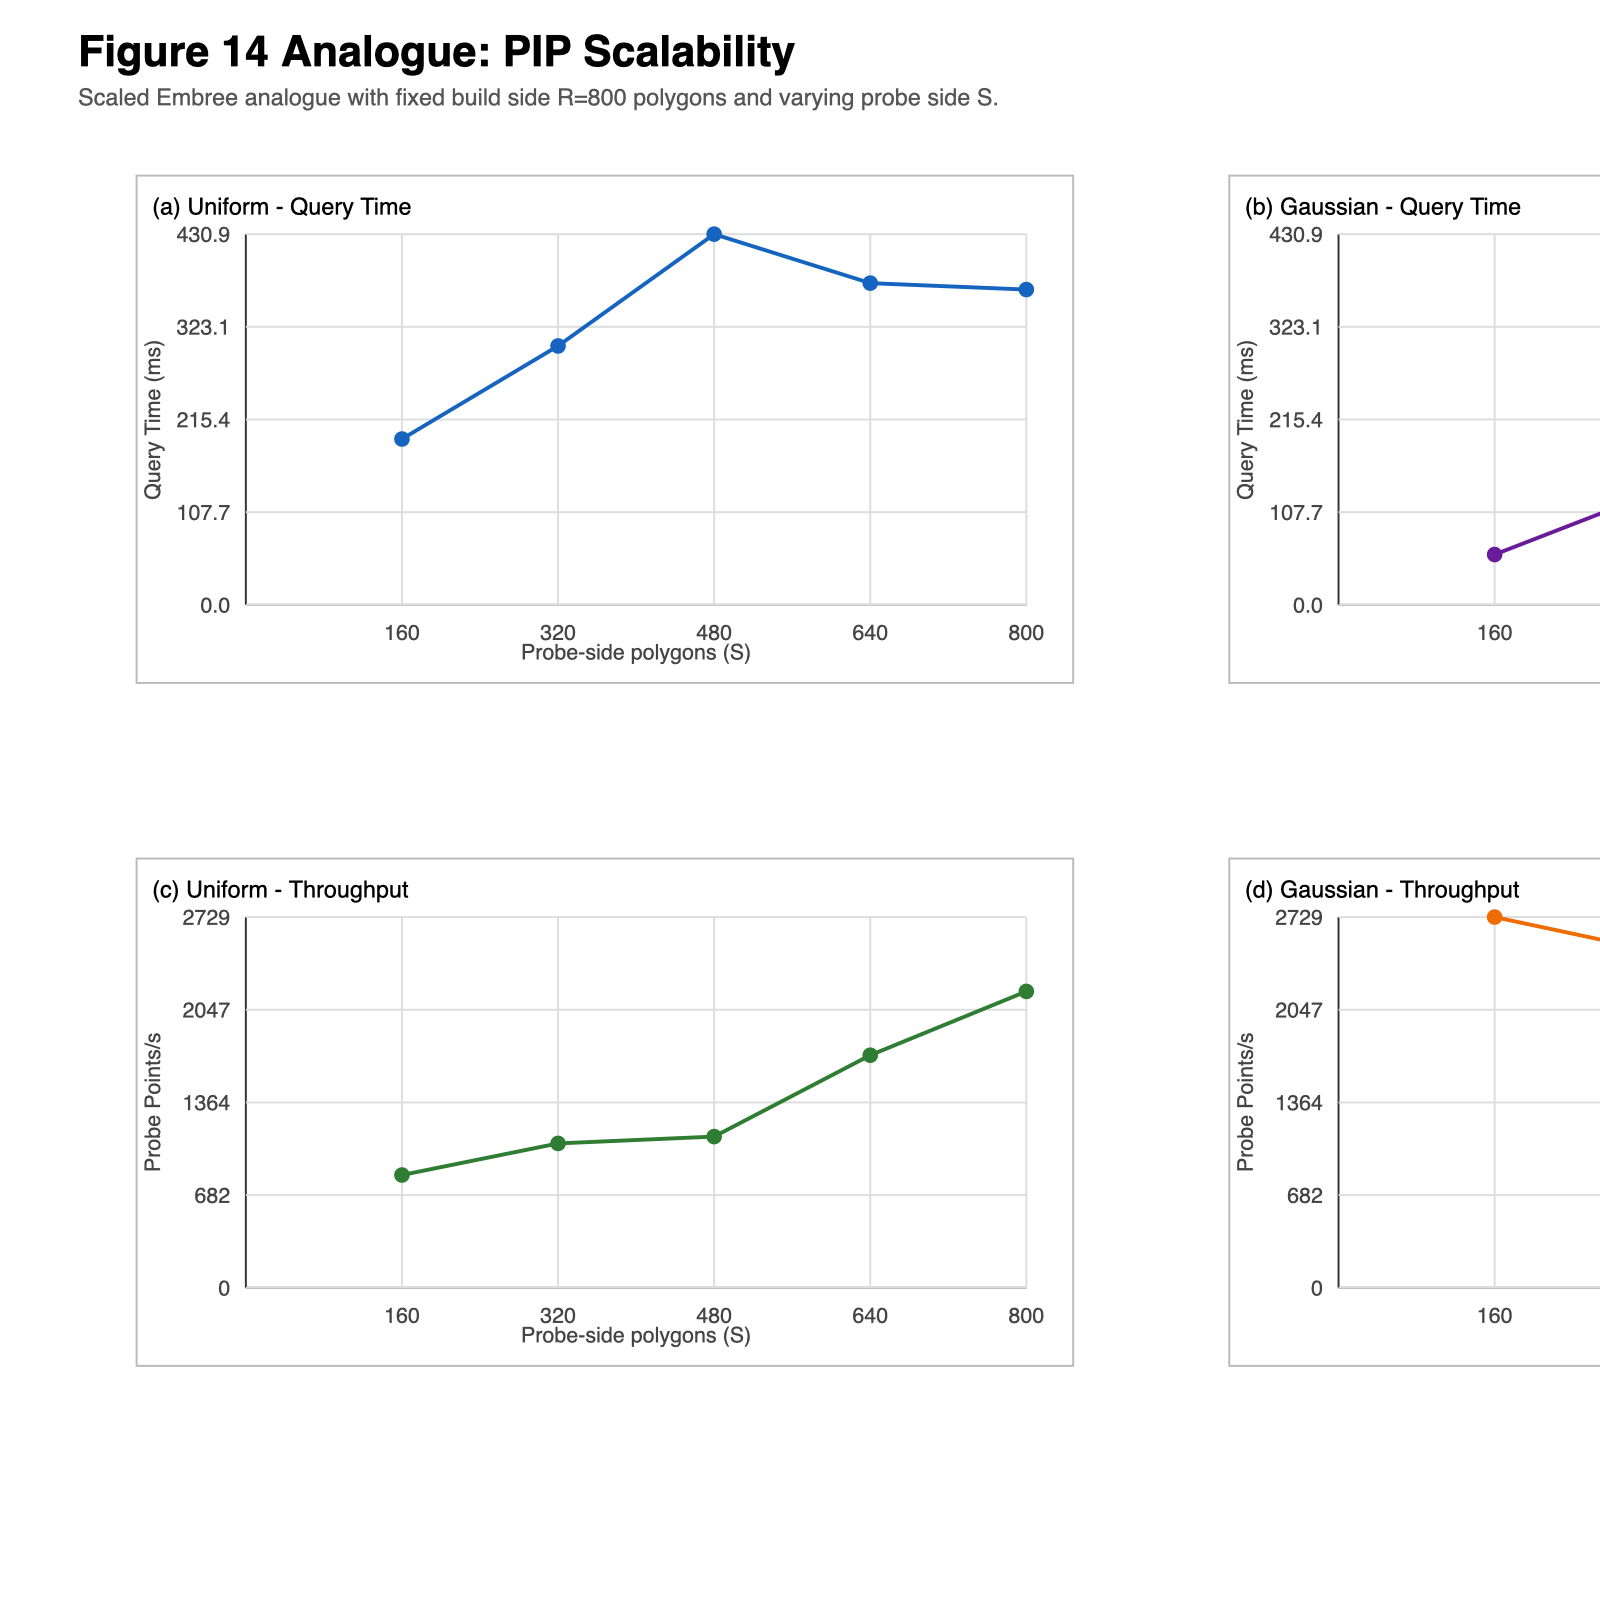
\includegraphics[width=0.48\textwidth]{figures/figure14_pip_scalability.png}
\caption{Accepted bounded analogues of the RayJoin Figure~13 (left, LSI scalability) and Figure~14 (right, PIP scalability) surfaces. These figures are not paper-scale reproductions; they are the accepted bounded synthetic analogues from the RTDL reproduction package.}
\label{fig:scalability}
\end{figure*}

\subsection{Performance Interpretation}

Figure~\ref{fig:overlay-speedup} summarizes the accepted RayJoin Figure~15-style
overlay speedup analogue. As with the rest of the overlay surface in this
paper, it is a bounded overlay-seed result rather than a full polygon overlay
materialization claim.

\begin{figure}[t]
\centering
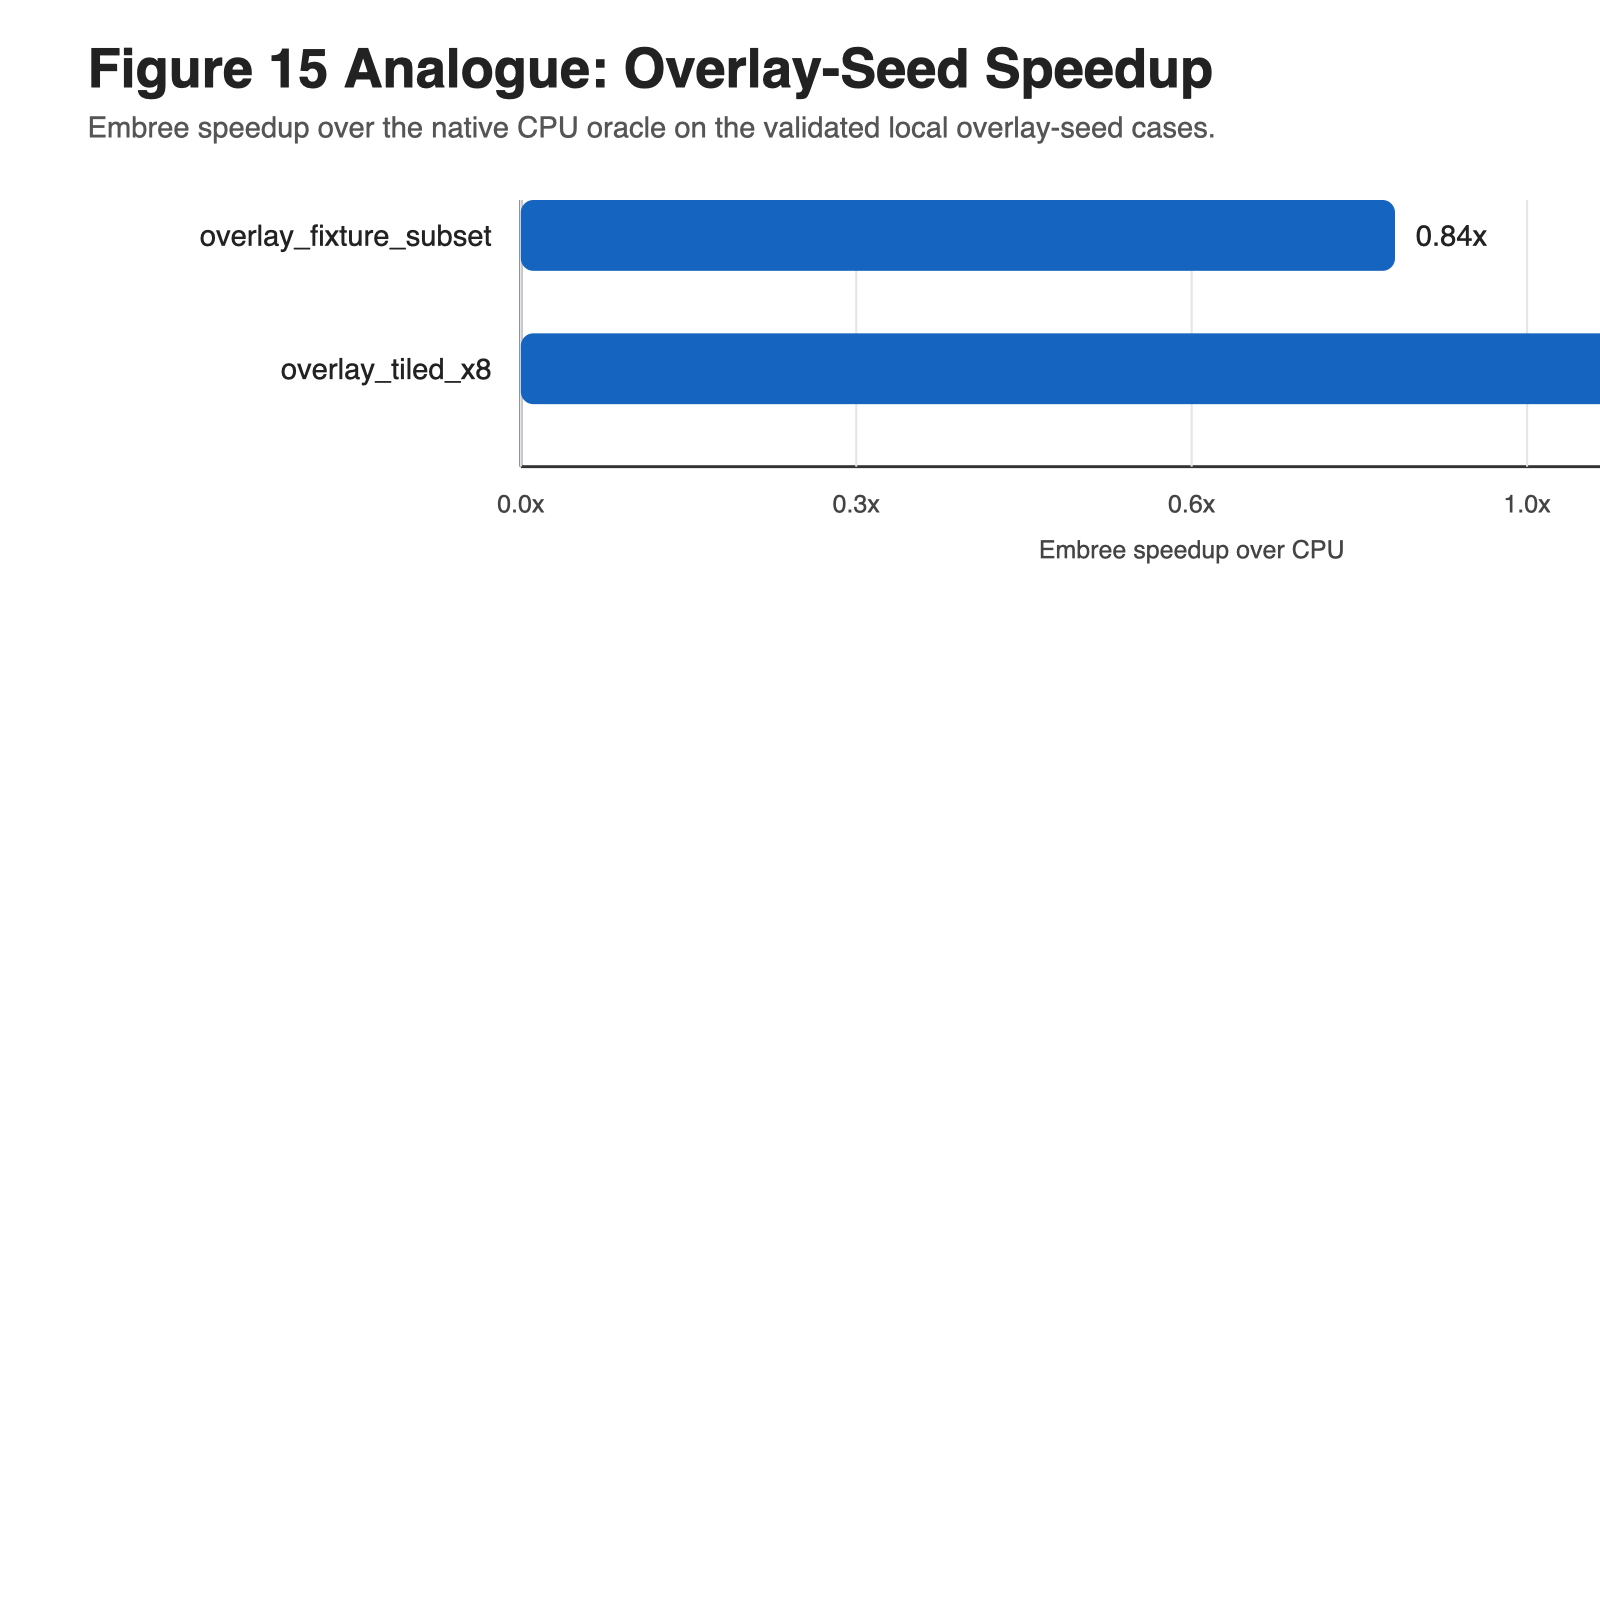
\includegraphics[width=\columnwidth]{figures/figure15_overlay_speedup.png}
\caption{Accepted bounded Figure~15-style overlay speedup analogue. The plotted surface corresponds to RTDL's current overlay-seed semantics, not full polygon overlay output geometry.}
\label{fig:overlay-speedup}
\end{figure}

The current results do not support a single universal backend winner. OptiX is
already beneficial on the largest accepted County/Zipcode package, but Embree
remains highly competitive and sometimes faster on smaller slices. PostGIS is
extremely fast on indexed positive-hit PIP queries, but the database and RTDL
are not executing identical end-to-end work because RTDL materializes full
truth rows while PostGIS is measured as an indexed hit query expanded into RTDL
equivalent truth for parity.

\section{How RTDL Mirrors the RayJoin Paper}

RTDL mirrors RayJoin along three important dimensions and then differs from it
in one explicit way.

\subsection{Workload Surface}

The paper-facing RTDL slice covers the same workload family categories that
matter to RayJoin:
LSI, PIP, and overlay composition.

\subsection{Artifact Structure}

RTDL now has a bounded paper-facing closure package covering:
\begin{itemize}
\item RayJoin Table~3 style bounded package rows,
\item RayJoin Figure~13 bounded scalability analogue (Figure~\ref{fig:scalability}, left),
\item RayJoin Figure~14 bounded scalability analogue (Figure~\ref{fig:scalability}, right),
\item RayJoin Table~4 bounded overlay-seed analogue,
\item RayJoin Figure~15 bounded overlay-seed speedup analogue (Figure~\ref{fig:overlay-speedup}).
\end{itemize}

\subsection{Evaluation Discipline}

The project mirrors the paper's experiment structure while replacing weak
claims with explicit fidelity labels. Rather than claiming unavailable or
unstable dataset families are done, RTDL defers them explicitly. Rather than
claiming full overlay materialization, RTDL labels the current closure as an
overlay-seed analogue. This produces a more reviewable and reproducible paper
story than an overstated “full reproduction” claim would.

\subsection{Key Differences from the Original Paper}

The current RTDL paper package differs from the original RayJoin paper in four
main ways:
\begin{enumerate}
\item It is bounded rather than paper-scale.
\item It relies on accepted analogues where exact paper data is unavailable.
\item It uses PostGIS as an external correctness reference, which RayJoin did
not use in the same way.
\item The current overlay surface is a seed-generation analogue, not full
polygon overlay materialization.
\end{enumerate}

\section{Limitations}

This work is intentionally explicit about its limitations.

First, this is not a paper-identical reproduction. Several continent-scale
lakes/parks families remain deferred because their public acquisition paths are
unstable or unavailable. In the current accepted package these deferred families
are:
\begin{itemize}
\item LKAF $\bowtie$ PKAF,
\item LKAS $\bowtie$ PKAS,
\item LKEU $\bowtie$ PKEU,
\item LKNA $\bowtie$ PKNA,
\item LKSA $\bowtie$ PKSA.
\end{itemize}

Second, the accepted practical analogue for the paper's \textit{Block
$\bowtie$ Water} row is the bounded \texttt{county2300\_s10} package over
BlockGroup and WaterBodies. That scoping qualifier matters and must not be
erased in downstream summaries.

Third, only bounded LKAU $\bowtie$ PKAU currently has four-system
overlay-seed closure. County/Zipcode and BlockGroup/WaterBodies remain useful
overlay analogue context from earlier Embree work, but not the same four-system
overlay closure.

Fourth, Vulkan is not part of the accepted paper package. It remains
provisional.

\section{Conclusion}

RTDL now supports a bounded, externally checked, multi-backend reproduction of
the RayJoin workload family that is strong enough to describe in paper form.
The current contribution is not a claim of full paper-identical reproduction.
Instead, it is a paper-facing bounded closure package grounded in accepted
evidence:
synthetic scalability analogues for RayJoin Figure~13 and Figure~14, bounded package
closure for the stable RayJoin Table~3 families, and bounded overlay-seed analogue
closure for RayJoin Table~4 and Figure~15. The result is a trustworthy baseline for
peer review and subsequent workload expansion, rather than a backend bring-up
story or a speculative full-reproduction claim.

\section*{Acknowledgment}

This manuscript is based on the current audited RTDL repository state and its
accepted multi-agent review process.

\bibliographystyle{IEEEtran}
\bibliography{references}

\end{document}
